\documentclass{standalone}
\usepackage{tikz}
\usepackage{amsmath}

\begin{document}
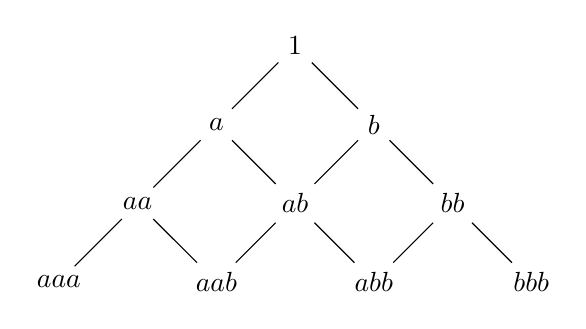
\begin{tikzpicture}
  \node (1) at (0,0) {$1$};
  \node (a) at (-1,-1) {$a$};
  \node (b) at (1,-1) {$b$};
  \node (aa) at (-2,-2) {$aa$};
  \node (ab) at (0,-2) {$ab$};
  \node (bb) at (2,-2) {$bb$};
  \node (aaa) at (-3,-3) {$aaa$};
  \node (aab) at (-1,-3) {$aab$};
  \node (abb) at (1,-3) {$abb$};
  \node (bbb) at (3,-3) {$bbb$};
  
  \draw (1) -- (a);
  \draw (1) -- (b);
  \draw (a) -- (aa);
  \draw (a) -- (ab);
  \draw (b) -- (ab);
  \draw (b) -- (bb);
  \draw (aa) -- (aaa);
  \draw (aa) -- (aab);
  \draw (ab) -- (aab);
  \draw (ab) -- (abb);
  \draw (bb) -- (abb);
  \draw (bb) -- (bbb);
\end{tikzpicture}
\end{document}